% interacttfqsample.tex
% v1.05 - August 2017

%\documentclass[]{interact}
\documentclass[sn-vancouver, Numbered]{sn-jnl}

\usepackage[table]{xcolor}
\usepackage{hyperref}
\usepackage{siunitx}

\usepackage{graphicx}%
\usepackage{multirow}%
\usepackage{amsmath,amssymb,amsfonts}%
\usepackage{amsthm}%
\usepackage{mathrsfs}%
\usepackage[title]{appendix}%
\usepackage{xcolor}%
\usepackage{textcomp}%
\usepackage{manyfoot}%
\usepackage{booktabs}%
\usepackage{algorithm}%
\usepackage{algorithmicx}%
\usepackage{algpseudocode}%
\usepackage{listings}%
%%%%

%%%%%=============================================================================%%%%
%%%%  Remarks: This template is provided to aid authors with the preparation
%%%%  of original research articles intended for submission to journals published 
%%%%  by Springer Nature. The guidance has been prepared in partnership with 
%%%%  production teams to conform to Springer Nature technical requirements. 
%%%%  Editorial and presentation requirements differ among journal portfolios and 
%%%%  research disciplines. You may find sections in this template are irrelevant 
%%%%  to your work and are empowered to omit any such section if allowed by the 
%%%%  journal you intend to submit to. The submission guidelines and policies 
%%%%  of the journal take precedence. A detailed User Manual is available in the 
%%%%  template package for technical guidance.
%%%%%=============================================================================%%%%

%%\unnumbered% uncomment this for unnumbered level heads
%\usepackage[caption=false]{subfig}% Support for small, `sub' figures and tables
%\usepackage[numbers,sort&compress]{natbib}% Citation support using natbib.sty
%\bibpunct[, ]{[}{]}{,}{n}{,}{,}% Citation support using natbib.sty
%\renewcommand\bibfont{\fontsize{10}{12}\selectfont}% Bibliography support using natbib.sty


\raggedbottom

\begin{document}

%\articletype{ARTICLE TEMPLATE}% Specify the article type or omit as appropriate

\title{MultIHeaTS : an Open Source Implicit Thermal Solver for 1D Multilayered Surfaces}

%\author{
%\name{C. Mergny\textsuperscript{a}\thanks{CONTACT Cyril Mergny, Email: cyril.mergny@universite-paris-saclay.fr} and F. Schmidt\textsuperscript{a,b}}

\author*[1]{\fnm{C.} \sur{Mergny}}\email{cyril.mergny@universite-paris-saclay.fr}
\author[1,2]{\fnm{F.} \sur{Schmidt}}\email{frederic.schmidt@universite-paris-saclay.fr}

\affil*[1]{\orgdiv{GEOPS}, \orgname{Paris-Saclay University}, \city{Orsay}, \country{France}}
\affil[2]{ \orgname{Institut Universitaire de France}, \city{paris}, \country{France}}





\abstract{An implicit Euler scheme is proposed for solving heat conduction problems in 1D  heterogeneous media, available as an open source Python code.
The algorithm uses finite difference on an irregular grid and is unconditionally stable due to the implicit formulation.
 The boundary conditions can be imposed either in temperatures or fluxes.
The thermal solver is validated against a stiff analytical solution, demonstrating its robustness in handling stiff equations.
 Its general applicability for heterogeneous cases is demonstrated through its use in a planetary surface scenario with non-linear boundary conditions induced by black body thermal emission.
The upper boundary condition is formulated explicitly, which introduces negligible errors while maintaining the scheme's stability. 
Although the Crank-Nicolson scheme is generally considered more reliable for homogeneous media, our numerical study shows that the proposed implicit scheme is more accurate for larger time steps in more realistic heterogeneous media, which is particularly relevant for the planetary science field.}




\keywords{
Heat Diffusion Equation; Implicit Finite Difference; Heterogeneous Surfaces; Non-Linear Boundary Condition; Open-Source Python
}

\maketitle

\section{Introduction}

The heat equation is a fundamental partial differential equation that governs the behavior of heat transfer in various physical systems. However, when dealing with heterogeneous media, where the thermal properties of the material vary spatially, the heat equation becomes too complex to solve analytically \cite{Jaeger1950, Loeb2019}. In one dimension, the heat equation for conduction transfers can be expressed as:
\begin{equation}
    \rho(x, t) c_{\mathrm{p}}(x, t) \dfrac{\partial T(x, t)}{\partial t} =  \dfrac{\partial}{\partial x} \left( k(x, t) \dfrac{\partial}{\partial x} T(x, t) \right)
    +  Q(x, t)
    \label{eq:heat-equation}
\end{equation}
where $x$ denotes space and $t$ denotes time, $T$ is the temperature, $\rho$ is the density, $c_{\mathrm{p}}$ is heat capacity, $k$ is thermal conductivity, and $Q$ denotes an optional source or sink term.
We propose to solve numerically the heat equation where all thermal properties can vary continuously over space and time, and with non-constant time and space increments.

Several numerical methods have been developed to solve the heat equation for heterogeneous media, including finite element and finite volume methods \cite{Roubicek1990, Lage1996, Nissen2017, Loeb2019, Masson2020}, finite difference schemes \cite{Spencer1989, Schorghofer2010}, and other methods \cite{Fudym2002, Fang2009}. 
In this paper, we focus on finite difference schemes due to their ease of implementation, making them more accessible for coupling with multi-physics simulations in further studies \cite{Langtangen2017}.

The target science case is in Earth and Planetary science with surface conditions subject to solar illumination. In this scenario, the upper boundary condition (i.e., the flux leaving the surface) is determined by the energy equilibrium between the solar flux and the black body emission from the surface \cite{Spencer1989}.
\begin{equation}
    \forall t, k(0,t) \left. \dfrac{\partial T(x, t)}{\partial x}\right|_{x=0} =  - F_{\mathrm{solar}}(t) + \epsilon \cdot \sigma_{\mathrm{SB}} \cdot T(0, t)^4
    \label{eq:energy-eq}
\end{equation}
where $\epsilon$ is the thermal emissivity and $\sigma_{\mathrm{SB}}$ the Stefan-Boltzmann constant.
A simplified model for solar illumination at the equator with zero obliquity throughout a sidereal day can be expressed as a truncated sinusoidal function \cite{Spencer1989} :
\begin{equation}
	F_{\mathrm{solar}}(t) = \left\{ 
		\begin{array}{ll}
			\left(1 - A \right) \dfrac{G_{\mathrm{SC}}}{d^2} \cos \left(\dfrac{2 \pi t}{P} \right) & \text{ if } {2 \pi t}/{P} \text{ in } \left[-\frac{\pi}{2}, \frac{\pi}{2}\right] \\ 
		\text{or} \\
		0   &  \text{ if }  {2 \pi t}/{P} \text{ in } \left]\frac{\pi}{2}, \frac{3\pi}{2}\right[ \\
		\end{array}
	\right.
\end{equation}
where $A$ is the surface albedo, $G_{\mathrm{SC}}$ the solar constant in W.m$^{-2}$ and $d$ the distance between the Sun and the planet in AU. 
It should be noted that while this simplified model captures the essential features of solar illumination, 
more realistic estimations, for instance from NASA's SPICE toolkit \cite{Acton1996, Acton2018} can be easily integrated.

In the planetary science context, various numerical models have been developed to study the behavior of both homogeneous surfaces \cite{Wesselink1948, Rozitis2011, Kieffer2013}, and heterogeneous media, as shown in Spencer's implementation of the explicit Euler scheme \cite{Spencer1989}. 
 Although the explicit method is easier to numerically implement and has a faster computational time per iteration, its main drawback is its conditional stability \cite{Press1992}.
A Crank-Nicolson scheme \cite{Crank1947} has been proposed by Schorgofer \cite{Schorghofer2010}. This scheme is more complex to implement and requires a computationally expensive matrix inversion. However, it offers the advantage of being unconditionally stable and more precise than first-order implicit and explicit schemes for homogeneous media, owing to its second-order truncation error in time \cite{Mazumder2016}.
 
 
 Although the implicit Euler scheme is also unconditionally stable, to our knowledge, there are no code available online that uses it to solve the heat equation in a heterogeneous media. 
 Therefore, our goal is to provide the scientific community with an open-source, easy-to-use, and versatile implicit solver called MultIHeaTS (Multi-layered Implicit Heat Transfer Solver) for solving the heat equation in such conditions. The source code is available online \footnote{MultIHeaTS open-source code available at \url{https://gitlab.dsi.universite-paris-saclay.fr/cyril.mergny/multiheats}}. Even though our target science is planetary science with surface conditions subject to solar illumination \cite{Wesselink1948, Spencer1989, Schorghofer2010, Rozitis2011, Kieffer2013}, this approach is applicable in a wide range of boundary conditions for a large set of scientific and technical cases.

In the first section of this article, we begin by presenting the mathematical derivation of the heat equation in heterogeneous media using the implicit Euler method. We then proceed to validate the MultIHeaTS algorithm by comparing its results to analytical solutions and other existing algorithms. Finally, we conduct a numerical study to evaluate the performance of the finite difference schemes under realistic planetary science conditions.

\section{Methods}


To discretize the heat equation, we used finite differences on an irregular spatial grid consisting of $n_x$ points, which we iterated for a total of $n_t$ iterations. The spatial and temporal parameters were discretized as follows:
\begin{equation}
\begin{cases}
    x \rightarrow x_n &= x_{n-1} + \Delta x_n \\
    t \rightarrow t^i &= t^{i-1} + \Delta t^i .\\
    
\end{cases}
\end{equation}
Here, $n$ is an integer such that $n \in \{0, \: \dotsc \: , n_x-1 \} $, representing the $n$th element in the spatial dimension, and $i$ is an integer such that $i \in \{0, \: \dotsc \: , n_t-1 \} $, representing the $i$th element in the time dimension. It is worth noting that both the spatial $\Delta x_n$ and temporal $\Delta t^i$ increments may not be constant.

\subsection{Backward Euler Finite Differences on an Irregular Grid}

Following the method described in \cite{Sundqvist1970}, the first order derivative of function $f$ using the central difference approximation can be written as :
\begin{equation}
\frac{\partial f}{\partial x} (x_n) = \frac{f_{n+1}- f_{n}}{2 \Delta x_n} + \frac{f_{n}- f_{n-1}}{2 \Delta x_{n-1}} + \mathcal{O}(\Delta x_n^2)
 \label{eq:1_deriv}
\end{equation}
and the second order derivative as :
\begin{equation}
	\frac{\partial f^2}{\partial x^2} = \dfrac{2 \left( f_{n+1} \Delta x_{n-1} + f_{n-1} \Delta x_{n} - f_n \left( \Delta x_{n} + \Delta x_{n-1}\right) \right) }{\Delta x_{n} \Delta x_{n-1} \left( \Delta x_{n} + \Delta x_{n-1}\right)} + \mathcal{O}(\Delta x_n^3)
 \label{eq:2_deriv}
\end{equation}


By using Equations \ref{eq:1_deriv} and \ref{eq:2_deriv}, the heat equation can be discretized with second order accuracy in space and first order in time. After factorizing each temperature term, the resulting equation is given by:
\begin{align}
\begin{split}
	T_n^i + r_n^i Q_n^i = &T_{n-1}^{i+1}  \left[ \frac{-r_n}{\Delta x_{n-1}} \left( - \frac{1}{2} \frac{\partial k}{ \partial x} + \frac{2 k_n}{\Delta x_n + \Delta x_{n-1}} \right)  \right] \\
	+ &T_{n}^{i+1} \left[ 1 - \frac{r_n}{\Delta x_{n}\Delta x_{n-1}} \left( \frac{\left(\Delta x_{n}- \Delta x_{n-1} \right)}{2} \frac{\partial k}{ \partial x} - 2 k_n \right) \right] \\
      + &T_{n+1}^{i+1}\left[ \frac{-r_n}{\Delta x_{n}} \left( \frac{1}{2} \frac{\partial k}{ \partial x} + \frac{2 k_n}{\Delta x_n + \Delta x_{n-1}} \right) \right]
\end{split}
    \label{eq:dis_heat}
\end{align}
with $r_n$ a coefficient expressed as $r_n^i = \Delta t^i / (\rho_n^i c_{\mathrm{p}, n}^i)$. With matrix notation this is equivalent to the system :
\begin{equation}
    \begin{pmatrix}
    b_0 & c_0 & &  &\hdots  & & 0  \\
    a_1 & b_1 & c_1 &  \\
      &\ddots & \ddots & \ddots     \\
    \vdots  &  & a_n & b_n & c_n & &  \vdots \\
    & & &\ddots & \ddots & \ddots     \\
    & & &  & a_{n_x-2} & b_{n_x-2} & c_{n_x-2} \\
    0 & &  \hdots & & & a_{n_x-1} & b_{n_x-1}  \\
    \end{pmatrix}
    \cdot
    \begin{pmatrix}
    T_{0} \\
    \vdots \\
    T_{n-1} \\
    T_{n}  \\
    T_{n+1} \\
    \vdots \\
    T_{n_x-1}
    \end{pmatrix}^{i+1}
     = 
     \begin{pmatrix}
        s_{0} \\
        \vdots \\
        s_{n-1} \\
        s_{n}  \\
        s_{n+1} \\
        \vdots \\
        s_{n_x-1}
        \end{pmatrix}^{i}
\end{equation}
where the coefficients $a_n$, $b_n$, $c_n$ and $s_n$ are given by
\begin{equation}
\forall n \in \{2, \dots, n_x-1 \ 
\begin{cases}
& a_n =   \dfrac{-r_n}{\Delta x_{n-1}} \left( - \dfrac{1}{2} \dfrac{\partial k}{ \partial x} + \dfrac{2 k_n}{\Delta x_n + \Delta x_{n-1}} \right) \\
& b_n = 1 - \dfrac{r_n}{\Delta x_{n}\Delta x_{n-1}} \left( \dfrac{\left(\Delta x_{n}- \Delta x_{n-1} \right)}{2} \dfrac{\partial k}{ \partial x} - 2 k_n \right) \\
& c_n =  \dfrac{-r_n}{\Delta x_{n}} \left( \frac{1}{2} \dfrac{\partial k}{ \partial x} + \dfrac{2 k_n}{\Delta x_n + \Delta x_{n-1}} \right)\\
& s_n = T_n^i + r_n^i Q_n^i\\
\end{cases}
\end{equation}
and by the boundary conditions.


\subsection{General Boundary Conditions}

MultIHeaTS accepts any type of boundary conditions, including imposed flux or imposed temperatures at the boundaries. A detailed derivation of the Dirichlet boundary conditions can be found in Supplementary Materials Section 1. In the case of planetary surface evolution, we are specifically interested in Neumann boundary conditions, which involve imposed flux. 
In this scenario, the flux is prescribed at the boundaries:
\begin{equation}
    \forall t, k_0 \left. \dfrac{\partial T(x, t)}{\partial x}\right|_{x_0} = \phi_0(t).
    \label{eq:upper_flux}
\end{equation}
By injecting Equation \ref{eq:upper_flux} into the discretized heat Equation \ref{eq:dis_heat}, the upper boundary condition becomes:
\begin{equation}
    T_0^{i+1} = T_0^i + r_0^i \left[ \Delta x_{0} \phi_0^{i+1} \left(k_{1}^i - 3k_{0}^i\right) + \Delta x^2_0 Q_0^i \right]
      +  2 r_0^i k_0^i T_{1}^{i+1} - 2 r_0^i k_0^i  T_{0}^{i+1}
\end{equation}
which gives the expression of the first coefficients of the tri-diagonal matrix :
\begin{equation}
    \begin{cases}
        &b_0 = 1 + 2 r_0 k_0 / \Delta x_0^2  \\
        &c_0 = - 2 r_0 k_0   / \Delta x_0^2 \\
        &s_0 =  T_0^i + r_0 \left( \phi_0 \left(k_{1} - 3k_{0} \right)/\Delta x_0 +  Q_0 \right) \\
    \end{cases}   
    \label{eq:coeff_up}
\end{equation}
The same reasoning can be applied to the bottom boundary condition :
\begin{equation}
    \forall t, \left. \dfrac{\partial T(x, t)}{\partial x}\right|_{x_{n_x-1}} = \phi_{n_x-1}(t) 
\end{equation}
%\begin{equation}
%T_N^{i+1} = T_N^i + r_N^i \left[  \Delta x \phi_N^{i+1} \left(3k_{N}^i - k_{N-1}^i\right)  +  \Delta x^2 Q_n^i\right]
%+  2k_N^i r_N^i T_{N-1}^{i} - 2k_N^i r_N^i T_{N}^{i}
%\end{equation}
which gives the expression of the last tri-diagonal coefficients :
\begin{equation}
    \begin{cases}
        &a_{n_x-1}^i = - 2k_{n_x-1}^i r_{n_x-1}^i  \\
        &b_{n_x-1}^i = 1 +  2k_{n_x-1}^i r_{n_x-1}^i  \\
        &s_{n_x-1}^i =T_{n_x-1}^i + r_{n_x-1}^i \left[  \Delta x_{n_x-1} \phi_{n_x-1}^{i+1} \left( 3 k_{n_x-1}^i - k_{n_x-2}^i\right)  +  \Delta x^2_{n_x-1} Q_{n_x-1}^i\right] \\
        
    \end{cases}   
\end{equation}


\subsection{Non-Linear Boundary Conditions}

When dealing with planetary-like surfaces, a non-linearity problem arises from the energy equilibrium described in Equation \ref{eq:energy-eq}. This non-linearity comes from the Stefan-Boltzmann law, which states that the surface flux $\phi$ is proportional to $T_0^4$, making it a non-linear function of temperature: 
\begin{equation}
    \phi(t, T_0) \propto T_0^4
\end{equation}

For the explicit scheme, the non-linearity in the surface flux does not pose any issue as the surface flux can be pre-calculated using the previous surface temperature $T_{0}^{i-1}$. However, for Crank-Nicolson and Backward Euler schemes, the non-linearity of the Stefan-Boltzmann law makes it impossible to solve the implicit formulation of the upper boundary conditions as given in Equation \ref{eq:coeff_up}. To circumvent this issue, Schorghofer proposed a workaround \cite{Schorghofer2010} by linearizing the black body emission around a reference temperature $T_{\mathrm{r}}$:
\begin{equation}
T_0 = \left( T_{\mathrm{r}} + \delta T \right)^4 \approx T_{\mathrm{r}}^4 + T_{\mathrm{r}}^3 \delta T
\end{equation}
However it should be noted that $T_{\mathrm{r}}$ is chosen to be equal to the previous surface temperature $T_0$, making this formulation explicit.
This approach led to the development of a new boundary condition formulation which is sensible to abrupt changes of energy input, causing the surface temperature to vary rapidly.
If the reference temperature is far from the actual surface temperature this causes a significant error in the evaluation of the emitted energy. To address this issue, Schorghofer \cite{Schorghofer2010} uses a predictor-corrector step that iteratively adjusts the reference temperature.

%\textcolor{red}{but it comes with issues \cite{Press1992} ?}

We choose to formulate the boundary surface flux explicitly for the MultIHeaTS solver, following the same approach as for the explicit Euler scheme. Our validation tests, discussed in Section \ref{sec:results}, demonstrate that this approach does not introduce large errors and the algorithm remains stable.
One advantage of the implicit Euler scheme is that an explicit formulation of the surface flux can be used, while maintaining stability and adding little to no errors \cite{Beam1982}. We propose that this robustness may be due to the strong damping of oscillations discussed in Section \ref{sec:stability}. 
Similar to Schorghofer's solver, the implicit scheme may encounter issues when there are abrupt changes in surface temperatures. Nonetheless, the scheme is capable of accurately estimating the upper boundary condition using an explicit method and maintaining stability.


\subsection{Stability and Accuracy of the Finite Difference Schemes in Homogeneous Media}
\label{sec:stability}

Before analyzing the behavior of finite difference schemes in heterogeneous media, it is instructive to perform a stability analysis in simpler homogeneous media.
We follow the Fourier transform approach as described in \cite{Pearson1965, Giles1995, Thomas1995, Oesterby2003, Langtangen2017}: by injecting wave components of different frequencies $\phi \in [-\pi, \pi]$ into the heat Equation \ref{eq:heat-equation}, we can look at the response and behavior of the different schemes.

The propagation of the finite difference solution from one time step to the next is governed by the growth factor which for the explicit method is:
\begin{equation}
    g(\phi) = 1 - 4 F \sin^2\dfrac{\phi}{2}
\end{equation}
where values of $\phi$ close to 0 indicate low frequency components and values close to $\pi$ indicate high oscillatory wave components and  $F$ is the Fourier number defined as: 
\begin{equation}
    F = \dfrac{\alpha \Delta t }{ \Delta x^2}
\end{equation}
The growth of numerical wave components occurs when the absolute value of $g(\phi)$ exceeds 1,  which for explicit scheme happens if $F > \frac{1}{2}$. This leads to the magnification of the corresponding wave component, indicating instability.
Consequently, the explicit scheme is numerically unstable, and its domain of stability is given by:
\begin{equation}
   F < 1/2 
\end{equation}
The same analysis for the Backward Euler scheme leads to a growth factor of:
\begin{equation}
    g(\phi) = \left( 1 + 4 F \sin^2 \dfrac{\phi}{2}   \right)^{-1}
\end{equation}
In this case, the growth factor is constrained by $\left| g(\phi) \right| \le 1$ for all $F$ and $\phi$, meaning that the implicit scheme is unconditionally stable.

Finally the growth factor of the Crank-Nicolson method is given by: 
\begin{equation}
    g(\phi) = \dfrac{1- 2 F \sin^2 \frac{\phi}{2}}{1+2F \sin^2 \frac{\phi}{2}}.
\end{equation}
It is clear that the Crank-Nicolson method is also unconditionally stable as $\left| g(\phi) \right| \le 1$ for all values of $F$ and $\phi$.
However we note that for high frequency components $\phi \to  \pm \pi$ then $g(\phi) \to -1$, especially for large $F$, meaning that these components are propagated as weakly damped oscillations.

Notably, the growth factor of the implicit scheme is relatively small for high Fourier Numbers, which means that the components that exhibit the most problematic behavior in the Crank-Nicolson method are the same components that are most effectively damped by the implicit method \cite{Oesterby2003}. Hence, while the Crank-Nicolson is second-order accurate it is \textit{generally} stable for large timesteps, which is said to be L-Stable \cite{Press1992}.
 Conversely, the Backward Euler is stable for arbitrarily large time-step, said to be strongly A-stable \cite{Beam1982}, although it is only first-order accurate.
This means that the MultIHeaTS solver is particularly valuable in the field of planetary sciences, where large timescales can restrict the precision of time steps.

%iThe two latter are popular since they are unconditionally stable irrespective of
%the magnitude of bμ, and Crank-Nicolson especially so being of second order in time.
%One drawback with Crank-Nicolson, however, is that the solution has a tendency to oscillate
%if there are jump discontinuities in the initial condition or between the initial
%condition and a boundary condition.

%The stability criteria of the explicit scheme is given by the Fourier Number :
%\begin{equation}
%F = \max_{i, n} \left( \dfrac{\alpha_n^i \Delta t^i}{\Delta x^2_n}  \right) < \dfrac{1}{2}
%\end{equation}
%where $\alpha$ is the thermal diffusivity defined as $\alpha = k/\rho c_{\mathrm{p}}$.




\section{Results}
\label{sec:results}
\subsection{Validation with an Analytical Solution}

Validation of our model using known analytical solutions of the heat equation can be achieved for homogeneous profiles only since no analytical solutions exist in the general case.
%In the case of constant conductivity, density and heat capacity the 1D heat equation can be solved analytically for a given set of initial and boundary conditions.
If we consider a stiff initial condition given by a step function defined on $[0, L]$ by the expression :
\begin{equation}
    \forall x \in [0, L], \, T(x, 0) = \left\{
\begin{array}{ll}
0, & \text{if } x < L/2 \\
1, &  \text{if } x \geq L/2.\\
\end{array}
    \right.
\label{eq:step_fct}
\end{equation}
then the analytical solution with zero-flux boundary conditions can be obtained (detailed derivation in Supplementary Materials Section 2) %\ref{sup:ana})
through Fourier series decomposition:
\begin{equation}
    T(x, t) = \frac{1}{2} - \sum_{j=1}^{+\infty} \frac{2}{\pi j} \sin\left(\frac{\pi j}{2}\right) \cos\left(\frac{\pi j x}{L}\right)    e^{-\alpha \left(\dfrac{ \pi j}{L} \right)^2 t}.
\end{equation}

\begin{figure}[htpb]
	\centering
	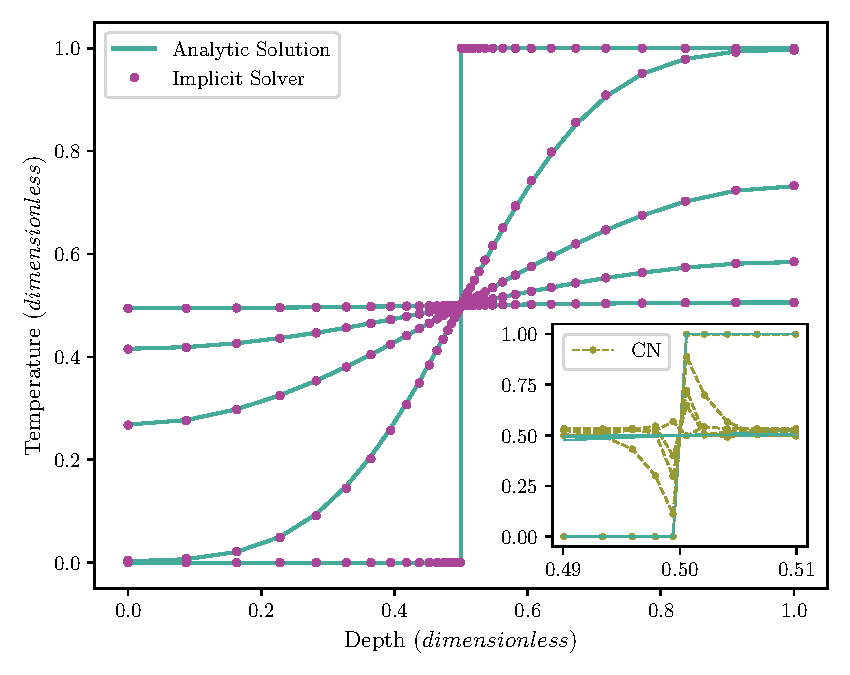
\includegraphics[width=0.8\textwidth]{valid_ana.pdf}
	\caption{Analytical validation for a stiff initial condition and homogeneous thermal properties on an irregular grid. Despite the discontinuity at $x = 0.5 $, the implicit solver MultIHeaTS can compute the evolution of temperature with a very close match  (maximum error $e_+< 0.5\%$) to the analytic solution. (\textit{Bottom Right}) Zoom on the spurious oscillations of the Crank-Nicolson solver at the location of the initial discontinuity. }
	\label{fig:valid_ana}
\end{figure}

To validate our model, we need to compare the computed temperatures with the analytical solutions for the same set of thermal parameters. This is done by computing the error, defined as the absolute value of difference between the temperature produced by the numerical model $T$ and the reference temperature $\theta$. The maximum error $e_+$ is expressed as : 
\begin{align}
    e_+ = \max_{n, i} \left| T^i_n - \theta^i_n \right|
\end{align}
and the average error $\overline{e}$ as :
\begin{equation}
    \overline{e} = \frac{1}{n_x n_t} \sum_{n, i}\left| T^i_n - \theta^i_n \right|
\end{equation}
with $\theta^i_n$ the reference temperature taken at the exact same location $x_n$ and time $t^i$.
For proper validation, both the numerical solver and the reference solution need to be calculated until the reach of a stationary regime, with exactly the same thermal properties and conditions (see Figure \ref{fig:valid_ana}). \
For a set of $n_x= 40$ grid points defining the box of length $L=\SI{1}{m}$ of constant diffusivity $\alpha \approx \SI{0.55}{m^2.s^{-1}}$ and $n_t=700$ iterations of timestep $\Delta t = \SI{2.3}{ms}$, the maximum error $e_+$ between the analytical solution and the implicit solver is less than 0.5\% and the mean error $\overline{e}$ is under 0.02\%.  
Results show a very close fit between the numerical and analytic solutions which proves that the MultIHeaTS model works well for homogeneous media.


The same test was performed using the Crank-Nicolson solver \cite{Schorghofer2010} to evaluate its ability to handle stiff initial conditions.
Using the same parameters as previously, the Crank-Nicolson solver produced spurious oscillations that were located around the initial discontinuity position (Figure \ref{fig:valid_ana}, \textit{Bottom Right}). 
The maximum error $e_+$ between the analytical solution and the Crank-Nicolson solver reaches up to 38\% and the mean error $\overline{e}$ averages 3\%. 
Although these oscillations eventually slowly disappear with time \cite{Oesterby2003}, it demonstrates that despite being the most accurate finite difference scheme, the Crank-Nicolson solver is less reliable in handling stiff initial conditions \cite{Press1992, Oesterby2003, Langtangen2017}, such as when two materials with different temperatures come into contact.


%\textcolor{red}{One drawback of CN is that it responds to jump discontinuities in the initial conditions with oscillations which are weakly damped and therefore may persist for a long time.  }


\subsection{Validation by Comparison with Explicit Scheme}

In more complex cases, in particular when the thermal conductivity vary with depth, the heat equation becomes too complex to solve analytically \cite{Jaeger1950}. 
In these cases, validation of the model is typically performed through comparison with experimental data and/or other well-established numerical algorithms.
Since our target application is the study of realistic planetary surface conditions, we decided to compare our method with Spencer's explicit scheme \cite{Spencer1989}, which is a commonly used algorithm in planetary science. 
Spencer's algorithm was implemented in IDL and can be obtained from his personal website \footnote{\url{https://www.boulder.swri.edu/~spencer/thermprojrs/}}.

%We used the same thermal properties, boundary conditions and numerical parameters (see Table. \ref{tab:params}), including the solar flux  $F_{\mathrm{solar}}$.

\begin{table}[htbp]
    \centering
    \begin{tabular}{ll}
    \toprule
    Parameters & Value \\ 
    \midrule
    Distance to Sun $d$ &  9.51 AU  \\
    Emissivity $\epsilon$ &  1  \\
    Albedo $A$ & 0.015  \\
    Grid points $n_x$ & 100  \\
    Max Depth   & 2 m    \\
    Initial Temperature $T$ &  90 K  \\
    Solar Period $P$  & 79.3 days   \\
    Number of Periods & 5   \\
    Number of iterations $n_t$ &  50000   \\
    Time Step $\Delta t$ &  685 s   \\
    \bottomrule
    \end{tabular}
\caption{Physics and numerical parameters used for comparing Spencer algorithm with MultIHeaTS.}
\label{tab:params}
\end{table}

\begin{table}[htbp]
    \centering
    \begin{tabular}{ l l c c l } 
     \toprule
     Thermal Properties & Unit & Top value & Bottom value & Interface \\ 
     \midrule
     Density $\rho$ & kg.m$^{-3}$ & 800 & 2000 & 25 cm \\ 
    Heat Capacity $c_{\mathrm{p}}$ & J.kg$^{-1}$.K$^{-1}$ & 600 & 1800 & 50 cm \\ 
    Inertia $I_{\mathrm{th}}$ & J.m$^{-2}$.K$^{-1}$.s$^{-1/2}$ & 200 & 20 & 100 cm \\ 
     \bottomrule
    \end{tabular}
\caption{Thermal properties of a bi-layered surfaced used for comparison of Spencer's explicit algorithm with MultIHeaTS. Although some of these values are close to what could be found on realistic icy surfaces, they were varied smoothly over large scales for validation purposes. }
\label{tab:thermal_ppties}
\end{table}

\begin{figure}[htpb]
	\centering
	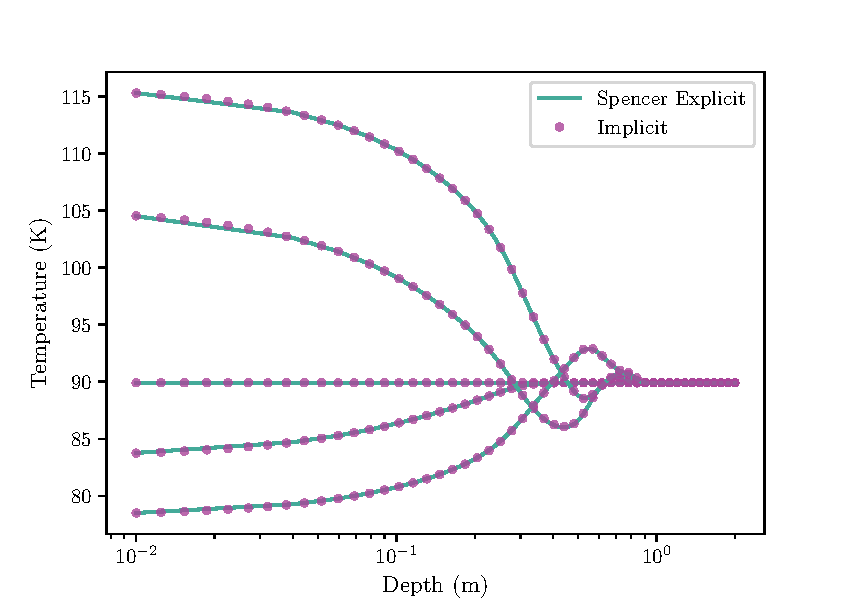
\includegraphics[width=0.8\textwidth]{valid_spencer.pdf}
	\caption{Validation of MultIHeaTS against Spencer's explicit algorithm. Temperature profiles for different times are plotted simultaneously $i = 0$, $20$, $159$, $300$, $699$. MultIHeaTS is as accurate as Spencer's explicit solver with the advantage of being unconditionally stable. 
    Note the uneven grid spacing of MultiHeaTS, denser at the surface, shown by the logarithmic horizontal axis.
    }
    \label{fig:val_spencer}
\end{figure}


Both algorithms were run with meticulous attention with the exact same thermal properties, boundary conditions, and numerical parameters that can be found in Table \ref{tab:params}.
For the sake of validation, values of density, heat capacity and conductivity are varied through the depth by the largest scales allowed by Spencer's explicit scheme stability criteria (see Table \ref{tab:thermal_ppties}).
 The MultIHeaTS solver exhibited a computational time of less than 1 minute on an Intel CPU i7-10750.


%on a $\SI{2}{m}$ thick grid consisting of $n_x=100$ points for $n_t = 5 \times 10^4 $ iterations, 

Overall, the results, presented in Figure \ref{fig:val_spencer},  show a very good similarity between the temperature profiles produced by the explicit and implicit schemes, with negligible differences between the two methods.
The maximum error between MultIHeaTS and the Spencer's solver is $e_+=0.68\%$ and the mean error is $\overline{e}=0.052\%$.
%\textcolor{red}{Errors are mostly concentred near the surface (in opposition to CN where they are at the highest temperature gradient, near the bi-layer interface.}
This comparison demonstrates that the MultIHeaTS solver can accurately compute temperature profiles for planetary surfaces, without the limitations of conditional stability that can be encountered with explicit methods.




\subsection{Comparison with Crank-Nicholson for Heterogeneous Media}

Another finite-differences implementation of the same heat transfer problem using the Crank-Nicolson scheme for heterogeneous planetary surfaces has been developed by Schorghofer \cite{Schorghofer2010} and is accessible online on his Github repository\footnote{\url{https://github.com/nschorgh/Planetary-Code-Collection}}. 
Unlike the explicit scheme, the Crank-Nicolson scheme is unconditionally stable and second-order accurate \cite{Mazumder2016}, which is an advantage in terms of accuracy and stability.   
However for more complex and realistic cases, such as heterogeneous surfaces subject to surface energy equilibrium,  it is unclear whether Crank-Nicolson remains the most reliable. 
In this section, we propose to evaluate the performance of the Crank-Nicolson scheme and our MultIHeaTS implicit scheme in comparison with the reference explicit solver outside the stability zone of the explicit algorithms. 
This will allow us to assess the reliability and accuracy of each scheme in simulating heat transfer in more challenging and realistic scenarios.

\begin{figure}[htpb]
	\centering
	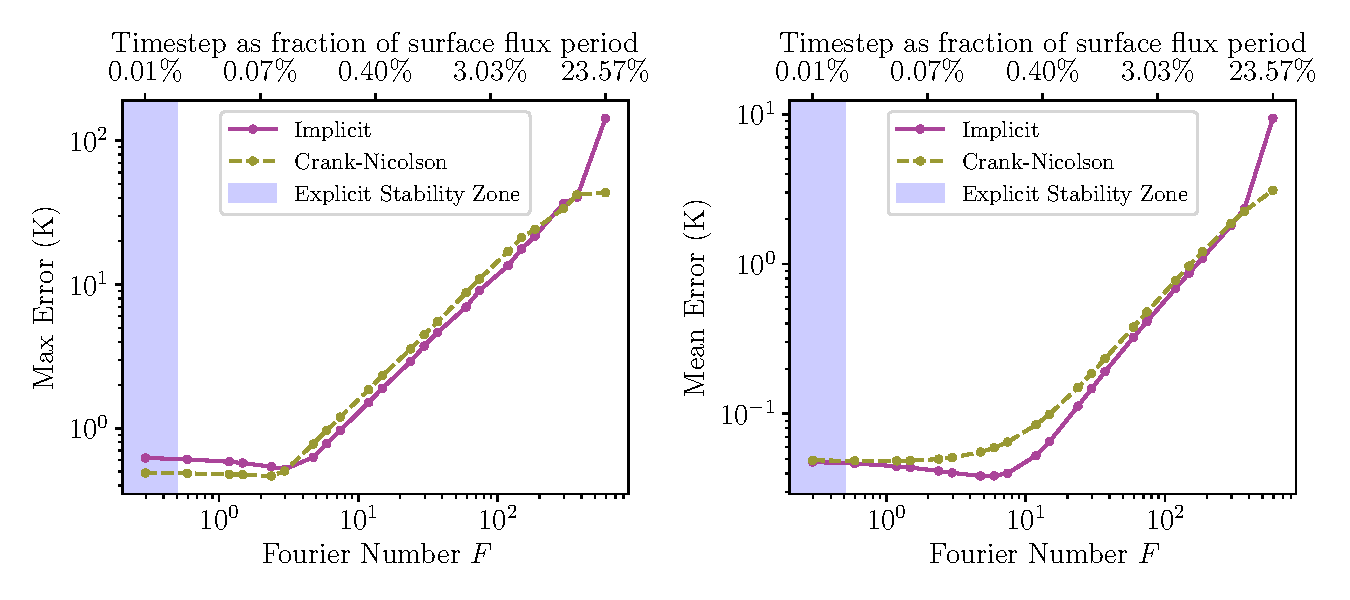
\includegraphics[width=1.0\textwidth]{solver_compare.pdf}
	\caption{Errors produced by the Crank-Nicholson and our MultIHeaTS implicit scheme in comparison to Spencer's explicit model as functions of the timesteps $\Delta t$ used (\textit{log-scales}). Average temperature is around $\SI{90}{K}$. Timestep $\Delta t$ is represented as a fraction of the surface flux' period at the top and by the Fourier number $F=\alpha \Delta t / \Delta x^2$ at the bottom. The stability zone of the explicit scheme $F< 1/2$ is represented in light blue. (Left) Maximum error $e_+$ produced by both solvers. (Right) Mean error $\overline{e}$ produced by both solvers. 
 }
	\label{fig:solvers_comp}
\end{figure}

To evaluate the effect of increasing timestep on the accuracy of our MultIHeaTS implicit scheme and the Crank-Nicolson scheme, we conducted a numerical experiment where we varied the timestep $\Delta t$ while keeping the grid and thermal properties fixed. We used Spencer's explicit algorithm with a small timestep $\Delta t = 2 \times 10^{-5}  P $ as a reference for the accurate computed temperatures. The properties and parameters used in this experiment are the same as for the previous experiments and can be found respectively on Table \ref{tab:params} and \ref{tab:thermal_ppties}. The increasing timestep causes the algorithms to lose information, leading to differences in the computed temperatures compared to Spencer's reference algorithm.




The results of our numerical experiment are presented in Figure \ref{fig:solvers_comp}. As expected, both the Crank-Nicholson and our MultIHeaTS implicit scheme are able to compute the temperature profile outside the stability zone ($F> 1/2$) but with increasing error as $F$ increases. 
We consider, arbitrarily, for maximum error larger than  $e_+ = 10 \%$ that algorithms are irrelevant.
We observe that the unconditional stability of both algorithms allows us to extend the domain of computation to about two orders of magnitude beyond the explicit stability limit, while keeping the error reasonably low. 

In all cases, we observed that the Crank Nicolson method is on average 30\% computationally faster per iteration than our implicit algorithm.
Near the explicit stability zone $F < 1/2$, both Schorghofer's Crank-Nicolson ($e_+=0.53\%$, $\overline{e} = 0.054\%$) and our MultiHeaTS algorithm ($e_+=0.68\%$, $\overline{e} = 0.052\%$) produced near equivalent results with a slightly lower maximum error for Crank-Nicolson. 
However, for larger timesteps at fixed grid and thermal properties, the difference in errors becomes more noticeable. 
Specifically, for $F$ values ranging from 1 to 100, the MultIHeaTS algorithm is more accurate on average and for the maximum error. For example, at $F = 60$, the maximum and mean errors for MultIHeaTS are $e_+ = 7.6 \%$ and $\overline{e} = 0.36\%$, respectively, while for Crank-Nicolson, the corresponding values are $e_+ = 9.6 \%$ and $\overline{e} = 0.42\%$. 
Beyond the $F=100$ threshold, the errors produced by both algorithms become too high for the output temperatures to be relevant.
%\textcolor{red}{Discuss why error decreases at first for implicit ? }


 The results of our study indicate that when working with timesteps that exceed the explicit stability zone, our implicit solver MultiHeaTS is equally reliable and may even be more accurate than the Crank-Nicolson solver. This finding is particularly relevant for planetary studies, where it is often necessary to analyze temperature variations over several years ($t^{n_t-1} \gg P$).
 In such scenarios, it is often computationally expensive to obtain a precise timestep for the diurnal evolution, emphasizing the importance of a more accurate solver capable of handling larger timesteps.
 

 



\section{Conclusion}
We have developed an open-source implicit algorithm called MultIHeaTS, which employs finite differences to solve the heat equation on 1D heterogeneous media with an irregular grid. While our primary focus is planetary science, our algorithm is adaptable and can accommodate different types of boundary conditions and surfaces.

For homogeneous cases, the algorithm was validated using a known analytical solution.
This validation which used a discontinuous initial equation showed the robustness MultIHeaTS to stiff equations, in contrary to the Crank-Nicolson method.
For heterogeneous cases, MultIHeaTS was validated by comparison to a well established explicit algorithm in planetary science \cite{Spencer1989}.
Despite our explicit formulation of the surface energy equilibrium condition, our implicit scheme remained accurate and stable, producing results that closely matched Spencer's model.
Thanks to its unconditional stability, this implicit Euler scheme allow us to extend the stability domain by two orders of magnitude, beyond which the truncation error becomes too significant ( $ e_+ > 10 \%$).

In a numerical study, we compared the errors produced by our algorithm with an existing implementation of the Crank-Nicolson scheme by Schorghofer \cite{Schorghofer2010}. Our results show that both models are equivalent for low Fourier numbers, and for higher Fourier numbers, our MultIHeaTS solver becomes more accurate than Crank-Nicolson.
For instance, at $F = 60$, the errors in MultIHeaTS are  $e_+ = 7.6 \%$ and $\overline{e} = 0.36\%$,  while for Crank-Nicolson, the corresponding errors are $e_+ = 9.6 \%$ and $\overline{e} = 0.42\%$.

Future research could investigate how the accuracy and stability of the MultIHeaTS algorithm are affected by the explicit formulation of the nonlinear upper boundary condition induced by black body emission. This would provide valuable insight into the behavior of the algorithm under more complex thermal conditions.

The MultIHeaTS algorithm has a wide range of potential applications, and its open-source and flexible nature make it adaptable to various domains. In planetary science, it is expected to be useful for retrieving thermal properties of multi-layered planetary surfaces using brightness temperature data. Moreover, due to its finite-difference formulation, it can be easily coupled with other physical processes to study, for example, the evolution of planetary icy surfaces.

\section*{Statements and Declarations}
\subsection*{Funding and Competing Interests}

We acknowledge support from the ``Institut National des Sciences de l'Univers'' (INSU), the ``Centre National de la Recherche Scientifique'' (CNRS) and ``Centre National d'Etudes Spatiales'' (CNES) through the ``Programme National de Plan{\'e}tologie''. 

The authors have no competing interests to declare that are relevant to the content of this article.

\section*{Data Availability}
The authors declare that the data supporting the findings of this study are available within the paper and on the online public repository  \url{https://gitlab.dsi.universite-paris-saclay.fr/cyril.mergny/multiheats}

%\newpage
%\section*{Figures}


\bibliography{library}

%
\section*{Appendices}

\subsection{Dirichlet boundary conditions:}
The temperature is fixed at the boundaries which gives us at the top boundary $x=a$:
\begin{equation}
    \forall t, T(a, t) = T_a(t) \implies
    \begin{cases}
        &b_1^i = 1 \\
        &c_1^i = 0 \\
        &s_1^i = T_a^i, \\
    \end{cases}  
\end{equation}
at at the bottom boundary $x=b$,
\begin{equation}
    \forall t, T(b, t) = T_b(t) \implies
    \begin{cases}
        &a_N^i = 0 \\
        &b_N^i = 1 \\
        &s_N^i = T_b^i. \\
    \end{cases}  
\end{equation}


\subsection{Analytic Solution}
\label{sup:ana}
\subsubsection{Fourier series}
Any periodical function $f$ in $\mathbb{R}$ of period $P$ can be written as a Fourier series:
\begin{equation}
    f(x) =  \frac{a_0}{2} + \sum_{n=1}^{+\infty} a_n \cos\left(\frac{2\pi n x}{P}\right) + b_n \sin\left(\frac{2\pi n x}{P}\right),
    \label{eq:fourier_series}
\end{equation}
with the coefficients $a_n$ and $b_n$ given by the expressions:
\begin{equation}
    a_n = \frac{2}{P} \int_P f(x) \cos\left(\frac{2\pi n x}{P}\right) dx,
    \label{eq:a_n}
\end{equation}
\begin{equation}
    b_n = \frac{2}{P} \int_P f(x) \sin\left(\frac{2\pi n x}{P}\right) dx.
    \label{eq:b_n}
\end{equation}
The expressions are obtained by integrating equation (\ref{eq:fourier_series}) as demonstrated here:
\begin{align*}
    \int_P f(x) \cos\left(\frac{2\pi m x}{P}\right) dx & =  \int_P  \cos\left(\frac{2\pi m x}{P}\right)\left[ \frac{a_0}{2} + \sum_{n=1}^{+\infty} a_n \cos\left(\frac{2\pi n x}{P}\right) + b_n \sin\left(\frac{2\pi n x}{P}\right) \right] dx \\
    &=  \sum_{n=1}^{+\infty} \int_P  a_n \cos\left(\frac{2\pi n x}{P}\right)  \cos\left(\frac{2\pi m x}{P}\right) dx \\
    &= a_m \frac{P}{2}
\end{align*}

\subsubsection{Fourier series of a step function}
Every function on a interval of length $P$ can be extended to a periodic function in $\mathbb{R}$ of period $P$.
First we will extend function $H$ on the interval $[-\frac{L}{2}, \frac{3L}{2}]$ such that the derivative at $x=0$ and $x=L$ are equal to zero (Boundary flux condition). 
The step function is still defined by equation (\ref{eq:step_fct}) in $[-\frac{L}{2}, \frac{3L}{2}]$.

Then we use equations (\ref{eq:a_n}) and (\ref{eq:b_n}) with $P=2L$ the interval length to find the coefficient $a_n$ and $b_n$:
\begin{align*}
    a_n &= \frac{1}{L} \int_{-\frac{L}{2}}^{\frac{3L}{2}} H(x) \cos\left(\frac{\pi n x}{L}\right) dx \\
    & = \frac{1}{L} \int_{\frac{L}{2}}^{\frac{3L}{2}} \cos\left(\frac{\pi n x}{L}\right) dx \\
    & = \frac{-2}{\pi n} \sin\left( \frac{\pi n}{2} \right)
\end{align*}
and a similar integration for $b_n$ leads to $b_n=0$.
The step function can then be written as a Fourier series using equation (\ref{eq:fourier_series}):
\begin{equation}
    H(x) = \frac{1}{2} - \sum_{n=1}^{+\infty} \frac{4}{\pi n} \sin\left(\frac{\pi n }{2} \right) \cos\left(\frac{\pi n x}{L}\right).
\end{equation}

\subsubsection{Solving the heat equation by separation of variables}

The solution of the 1D heat equation (\ref{eq:1Dheateq}) with initial condition (\ref{eq:step_fct}), can be obtained by separation of variables. Let's assume that the solution can be written as
\begin{equation}
    T(x, t) = v(x)w(t)
\end{equation}
with $v$ and $w$ functions of $x$ and respectively $t$. This expression injected int the heat equation results to:
\begin{equation}
   v(x) \dfrac{\partial w(t)}{\partial t} = \alpha  \dfrac{\partial^2 v(x)}{\partial x^2} w(t)
\end{equation}
This first order differential equation as for $w$ the general solution:
\begin{equation}
    w(t) = w(0) e^{\alpha \dfrac{v^{''}(x)}{v(x)} t}
\end{equation}
where $v^{''}$ is the second derivative of $v$ with respect to $x$. If we take $v(x) = T_n(x, 0) = f_n(x)$ the initial function decomposed in 
a Fourier series, then we have:
\begin{equation}
        v^{''}(x) = -\left(\frac{2 \pi n}{P} \right)^2 f_n(x)
\end{equation} 
and 
\begin{align*}
    & T(x, 0) = v(x)w(0) = f(x) \\
    & v(x) = f(x) \implies w(0) = 1
\end{align*}
which give us the exact express of the solution of $w$ with:
\begin{equation}
    w(t) = e^{-\alpha \left(\dfrac{2 \pi n}{P} \right)^2 t}
\end{equation}
Hence the solution is given by:

\begin{equation}
    T(x, t) = \frac{a_0}{2} + \sum_{n=1}^{+\infty} \left(a_n \cos\left(\frac{2\pi n x}{P}\right) + b_n \sin\left(\frac{2\pi n x}{P}\right) \right)  e^{-\alpha \left(\dfrac{2 \pi n}{P} \right)^2 t}
\end{equation}

\subsection{Parameters}
\begin{table}[htbp]
    \centering
    \begin{tabular}{ll}
    \hline
    Parameters & Value \\ 
    \hline
    Distance to Sun $d$ &  9.51 UA  \\
    Emissivity &  1  \\
    Albedo $A$ & 0.015  \\
    Grid points $n_x$ & 100  \\
    Max Depth  m & 2 m    \\
    Initial Temperature &  90 K  \\
    Solar Period $P$$  & 79.3 days   \\
    Number of Periods & 5   \\
    Number of iterations $n_t$ &   50000   \\
    \hline
    \end{tabular}
\caption{Physics and numerical parameters used for comparing Spencer algorithm with MultIHeaTS.}
\label{tab:params}
\end{table}




\end{document}
